%% abtex2-modelo-trabalho-academico.tex, v-1.9.6 laurocesar
%% Copyright 2012-2016 by abnTeX2 group at http://www.abntex.net.br/ 
%%
%% This work may be distributed and/or modified under the
%% conditions of the LaTeX Project Public License, either version 1.3
%% of this license or (at your option) any later version.
%% The latest version of this license is in
%%   http://www.latex-project.org/lppl.txt
%% and version 1.3 or later is part of all distributions of LaTeX
%% version 2005/12/01 or later.
%%
%% This work has the LPPL maintenance status `maintained'.
%% 
%% The Current Maintainer of this work is the abnTeX2 team, led
%% by Lauro César Araujo. Further information are available on 
%% http://www.abntex.net.br/
%%
%% This work consists of the files abntex2-modelo-trabalho-academico.tex,
%% abntex2-modelo-include-comandos and abntex2-modelo-references.bib
%%

% ------------------------------------------------------------------------
% ------------------------------------------------------------------------
% abnTeX2: Modelo de Trabalho Academico (tese de doutorado, dissertacao de
% mestrado e trabalhos monograficos em geral) em conformidade com 
% ABNT NBR 14724:2011: Informacao e documentacao - Trabalhos academicos -
% Apresentacao
% ------------------------------------------------------------------------
% ------------------------------------------------------------------------

\documentclass[
	% -- opções da classe memoir --
	12pt,				% tamanho da fonte
	openright,			% capítulos começam em pág ímpar (insere página vazia caso preciso)
	twoside,			% para impressão em recto e verso. Oposto a oneside
	a4paper,			% tamanho do papel. 
	% -- opções da classe abntex2 --
	%chapter=TITLE,		% títulos de capítulos convertidos em letras maiúsculas
	%section=TITLE,		% títulos de seções convertidos em letras maiúsculas
	%subsection=TITLE,	% títulos de subseções convertidos em letras maiúsculas
	%subsubsection=TITLE,% títulos de subsubseções convertidos em letras maiúsculas
	% -- opções do pacote babel --
	english,			% idioma adicional para hifenização
	french,				% idioma adicional para hifenização
	spanish,			% idioma adicional para hifenização
	brazil				% o último idioma é o principal do documento
	]{abntex2}

% ---
% Pacotes básicos 
% ---
\usepackage{lmodern}			% Usa a fonte Latin Modern			
\usepackage[T1]{fontenc}		% Selecao de codigos de fonte.
\usepackage[utf8]{inputenc}		% Codificacao do documento (conversão automática dos acentos)
\usepackage{lastpage}			% Usado pela Ficha catalográfica
\usepackage{indentfirst}		% Indenta o primeiro parágrafo de cada seção.
\usepackage{color}				% Controle das cores
\usepackage{graphicx}			% Inclusão de gráficos
\usepackage{microtype} 			% para melhorias de justificação
\usepackage{import}
% ---
		
% ---
% Pacotes adicionais, usados apenas no âmbito do Modelo Canônico do abnteX2
% ---
\usepackage{lipsum}				% para geração de dummy text
% ---

% ---
% Pacotes de citações
% ---
\usepackage[brazilian,hyperpageref]{backref}	 % Paginas com as citações na bibl
\usepackage[alf]{abntex2cite}	% Citações padrão ABNT
\usepackage{amsmath}
\usepackage{tikz}
\usepackage{graphicx}
\graphicspath{ {img/} }

\usepackage{lscape}
% --- 
% CONFIGURAÇÕES DE PACOTES
% --- 

% ---
% Configurações do pacote backref
% Usado sem a opção hyperpageref de backref
\renewcommand{\backrefpagesname}{Citado na(s) página(s):~}
% Texto padrão antes do número das páginas
\renewcommand{\backref}{}
% Define os textos da citação
\renewcommand*{\backrefalt}[4]{
	\ifcase #1 %
		Nenhuma citação no texto.%
	\or
		Citado na página #2.%
	\else
		Citado #1 vezes nas páginas #2.%
	\fi}%
% ---

% ---
% Informações de dados para CAPA e FOLHA DE ROSTO
% ---
\titulo{Segmentação e classificação de Big Data}
\autor{Gustavo Kendi Tsuji}
\local{São Paulo}
\data{2016}
\orientador{Alessandra Montini}
\instituicao{%
  Universidade de São Paulo - USP
  \par
  Faculdade de Economia, Administração e Ciências Contábeis - FEAUSP
  \par
  Bacharelado em Administração}
\tipotrabalho{Trabalho de Conclusão de Curso}
% O preambulo deve conter o tipo do trabalho, o objetivo, 
% o nome da instituição e a área de concentração 
\preambulo{Experimento quantitativo sobre algoritmos de segmentação e classificação para grandes bases de dados}
% ---


\input{structure/config.tex}
% ---
% compila o indice
% ---
\makeindex
% ---

% ----
% Início do documento
% ----
\begin{document}

% Seleciona o idioma do documento (conforme pacotes do babel)
%\selectlanguage{english}
\selectlanguage{brazil}

% Retira espaço extra obsoleto entre as frases.
\frenchspacing 

% ----------------------------------------------------------
% ELEMENTOS PRÉ-TEXTUAIS
% ----------------------------------------------------------
% \pretextual

% ---
% Capa
% ---
\imprimircapa
% ---

% ---
% Folha de rosto
% (o * indica que haverá a ficha bibliográfica)
% ---
\imprimirfolhaderosto*
% ---

\input{structure/fichacategorica.tex}

\input{structure/errata.tex}

\input{structure/folhaaprovacao.tex}

\input{structure/dedicatoria.tex}

% ---
% Agradecimentos
% ---
\begin{agradecimentos}
Gostaria de agradecer a professora Alessandra Montini pelo apoio e orientação durante os estudos sobre um tema que tenho muito interesse em continuar aprendendo.

Também gostaria de agradecer a minha família que sem dúvidas me deram o suporte para que pudesse estudar e em especial, a minha noiva Eliana que sempre esteve ao meu lado.

\end{agradecimentos}
% ---s

% ---
% Epígrafe
% ---
\begin{epigrafe}
    \vspace*{\fill}
	\begin{flushright}
		\textit{``One’s mind, once stretched by a new idea, \\
		 never regains its original dimensions. \\
		(HOMES, Oliver Wendell)}
	\end{flushright}
\end{epigrafe}
% ---

% ---
% RESUMOS
% ---

% resumo em português
\setlength{\absparsep}{18pt} % ajusta o espaçamento dos parágrafos do resumo

\begin{resumo}
 
 Nos dias atuais, a informação se tornou um recurso estratégico, crucial para toda empresa que busque competitividade no mercado. A sistematização e estudos de indicadores estão cada vez mais viavéis por conta da evolução tecnológica, que facilitou a acessibilidade de dessas informações. É a era do Big Data. Com os dados internos da empresa e externos do mercado é possível construir indicadores que podem dar norte a decisões . Em paralelo a isso, algoritmos de Machine Learning auxiliam a tarefa de compreender diversos aspectos explícitos e implícitos da empresa.

 \textbf{Palavras-chave}: Big Data. K Médias. Regressão Logística. Random Forest 
\end{resumo}

% resumo em inglês
\begin{resumo}[Abstract]
 \begin{otherlanguage*}{english}
In nowadays, the information has become a strategic resource, crucial to every company which seeks market competitiveness. The systematization and KPI studies are more viable because of technological evolution which has created facilities to retrieve those information. It is the Big Data era. With internal company and market external data it is possible to build KPI that can guide every decision. At the same time, machine learning algorithms aid to understand several explicit and implict company's aspects 

   \vspace{\onelineskip}
 
   \noindent 
   \textbf{Keywords}: : Big Data. K Means. logistic Regression. Random Forest
 \end{otherlanguage*}
\end{resumo}

\input{structure/listas/figuras.tex}

\input{structure/listas/tabelas.tex}

\input{structure/listas/siglas.tex}

\input{structure/listas/simbolos.tex}


% ---
% inserir o sumario
% ---
\pdfbookmark[0]{\contentsname}{toc}
\tableofcontents*
\cleardoublepage
% ---



% ----------------------------------------------------------
% ELEMENTOS TEXTUAIS
% ----------------------------------------------------------
\textual

% ----------------------------------------------------------
% Introdução (exemplo de capítulo sem numeração, mas presente no Sumário)
% ----------------------------------------------------------
\chapter*[Introdução]{Introdução}
\addcontentsline{toc}{chapter}{Introdução}
% ----------------------------------------------------------

A tecnologia evoluiu a ponto de tornar possível o armazenamento de volume de dados um grande desafio. Na internet, é possível encontrar mais de 60 trilhões de páginas indexadas pelo Google \cite{GOO01}. Só o Facebook possui warehouse com mais de 300 petabytes, tendo um tráfego de mais de 600 terabytes diários \cite{FAC01}.

Por trás desses dados brutos armazenados de forma estruturada ou não, existe o que \citeonline{BAEZA} chama de informação. Em geral, os dados são objetos brutos que trazem pouco ou nenhum significado. A informação, então, refere-se a uma interpretação do dado dentro de um contexto com um ganho cognitivo. A utilização dessa informação para qualquer fim produz o conhecimento. 

Por conta da dificuldade computacional em não só armazenar como analisar e monitorar esse volume de dados que nasceu o Big Data. 

Este trabalho visa estudar conceitos teóricos estatísticos que analisam os dados, os algoritmos que criam as informações, bem como tecnologias que auxiliam o processo como um todo.

Este documento e seu código-fonte são exemplos de referência de uso da classe
\textsf{abntex2} e do pacote \textsf{abntex2cite}. O documento 
exemplifica a elaboração de trabalho acadêmico (tese, dissertação e outros do
gênero) produzido conforme a ABNT NBR 14724:2011 \emph{Informação e documentação
- Trabalhos acadêmicos - Apresentação}.

A expressão ``Modelo Canônico'' é utilizada para indicar que \abnTeX\ não é
modelo específico de nenhuma universidade ou instituição, mas que implementa tão
somente os requisitos das normas da ABNT. Uma lista completa das normas
observadas pelo \abnTeX\ é apresentada em \citeonline{abntex2classe}.

Sinta-se convidado a participar do projeto \abnTeX! Acesse o site do projeto em
\url{http://www.abntex.net.br/}. Também fique livre para conhecer,
estudar, alterar e redistribuir o trabalho do \abnTeX, desde que os arquivos
modificados tenham seus nomes alterados e que os créditos sejam dados aos
autores originais, nos termos da ``The \LaTeX\ Project Public
License''\footnote{\url{http://www.latex-project.org/lppl.txt}}.

Encorajamos que sejam realizadas customizações específicas deste exemplo para
universidades e outras instituições --- como capas, folha de aprovação, etc.
Porém, recomendamos que ao invés de se alterar diretamente os arquivos do
\abnTeX, distribua-se arquivos com as respectivas customizações.
Isso permite que futuras versões do \abnTeX~não se tornem automaticamente
incompatíveis com as customizações promovidas. Consulte
\citeonline{abntex2-wiki-como-customizar} par mais informações.

Este documento deve ser utilizado como complemento dos manuais do \abnTeX\ 
\cite{abntex2classe,abntex2cite,abntex2cite-alf} e da classe \textsf{memoir}
\cite{memoir}. 

Esperamos, sinceramente, que o \abnTeX\ aprimore a qualidade do trabalho que
você produzirá, de modo que o principal esforço seja concentrado no principal:
na contribuição científica.

Equipe \abnTeX 

Lauro César Araujo



% ----------------------------------------------------------
% PARTE
% ----------------------------------------------------------
\part{Preparação da pesquisa}

Este trabalho se baseia em um experimento quantitativo sobre problemas relacionados a segmentação e classificação de dados de uma base de dados grande, utilizando algoritmos de K médias, regressão logística e random forest. Serão feitas interpretações, análises e comparações, levantando aspectos positivos e negativos de cada metodologia.

\begin{landscape}
\centering
\begin{vplace}[0.7]
\includegraphics[width=\textwidth]{gantt}
\end{vplace}
\end{landscape}

% ----------------------------------------------------------


% ---
% Capitulo com exemplos de comandos inseridos de arquivo externo 
% ---
\include{abntex2-modelo-include-comandos}
% ---

% ----------------------------------------------------------
% PARTE
% ----------------------------------------------------------
\part{Referenciais teóricos}
% ----------------------------------------------------------

% ---
% Capitulo de revisão de literatura
% ---
\chapter{Big Data}
% ---
\begin{mdframed}[backgroundcolor=blue!20] 
        Aqui pensei em colocar uma rápida introdução (não deve passar de 1 página) sobre caracaterísticas e/ou evolução do Big Data para poder contextualizar o problema em si e aplicação dos algoritmos em estudo
\end{mdframed}

\begin{comment}
O Big Data não representa apenas uma simples combinação de tecnologias.

Big Data possui três características intrínsicas: volume, velocidade e variedade.
\end{comment}

\subsection{Segmentação}


Com um volume de dados grande disponível, uma possibilidade para as empresas é conseguir reconhecer certos padrões. Por exemplo, conhecendo o perfil dos clientes, é possível adotar estratégias adequadas para cada segmento, principalmente quando o público alvo é composto por clientes muito heterogêneos. Segundo \citeonline[p. 257]{KOTLER}, ``segmentação de mercado é o ato de dividir um mercado em grupos distintos de compradores com diferentes necessidades e respostas''.

\begin{citacao} 
Um bom agrupamento exibe a característica de que objetos associados ao mesmo grupo são bastante similares, ao mesmo tempo em que objetos associados a grupos diferentes exibem uma baixa similaridade. Aplicações diretas da análise de grupos incluem segmentação de clientes ou de produtos, agrupamento de genes em um experimento de micro-array, organização dos resultados de uma consulta enviada a um mecanismo de busca da WEB, etc.
\cite{BEZERRA} \end{citacao}

Com a segmentação e os grupos definidos, é possível realizar uma análise descritiva para traçar um padrão no comportamento dos dados. 

% ---
\subsubsection{K Médias}
% ---

O K Médias é um algoritmo de \emph{machine learning} não supervisionado relativamente simples, podendo ser utilizado para resolver problemas de clusterização. Para \citeonline{MacQueen}, trata-se de um método que tem para uma quantidade k de \emph{clusters} pré definida, o objetivo de definir k centróides\footnotemark \footnotetext{centróide é um conceito muito utilizado em geometria e física e representa um ponto médio ou um centro de massa de uma representação. No caso de K Médias, considerando que as informações são transformadas em vetores, seria um ponto médio da informação}, um para cada \emph{cluster}, tal que o conjunto de dados possa ser repartido de forma eficiente. Para um conjunto de observações \begin{math}(x_{1}, x_{2}, ..., x_{n})\end{math}, onde 

\begin{equation}
\label{eq:media}
\underset{S}{\arg\min} \sum_{i=1}^{k} \sum_{x \in S_{i}}\left \| x - \mu_{i} \right \|^{2},
\end{equation}

onde \begin{math}\mu_{i}\end{math} é a média dos pontos em \begin{math}S_{i}\end{math}

O algoritmo minimiza a função objetiva usando o princípio dos mínimos quadrados. Por conta disso, é sensível a \emph{ouliers} e ruídos. O pseudo algoritmo do K Médias seria estes passos:\\

\begin{algorithm}[H]
\SetAlgoLined
 1. Defina uma inicialização inicial aleatória usando k \emph{clusters}\;
 \While{Não houve convergência}{
   2. Atribua para cada ponto do conjunto de dados um \emph{cluster} mais próximo\;
   3. Redefina a posição do centróide de cada \emph{cluster} como um ponto médio de todos os pontos do \emph{cluster}\;
 }
 \caption{K Médias}
\end{algorithm}

\vspace{5mm}


\begin{figure}[!ht]
\caption{Evolução da execução do algoritmo de K Médias }
\centerline{\includegraphics[width=0.5\textwidth]{img/k-means}}
\fonte{Extraído de \cite{kmeans-step}}
\end{figure}



A localização desses centróides deve ser o mais afastado entre si possível. A partir de uma posição inicial dos centróides, o próximo passo é, então, associar todos pontos do conjunto de dados com o centróide mais próximo. Com os pontos associados, recalcula-se k novos centróides como baricentros dos \emph{clusters} anteriores, repetindo esses passos até que os novos centróides sejam gerados muito próximos do passo anterior. 





% ---
\section{Classificação}
% ---

A classificação é uma análise preditiva com o objetivo de estabelecer modelos que possbilitem uma previsão do futuro, permitindo estudar tendências por meio do uso de técnicas estatísticas sobre dados históricos.

\subsection{Regressão Linear}


A regressão linear é uma modelagem matemática \footnotemark \footnotetext{modelagem matemática é uma representação em fórmulas matemáticas que tentam descrever ou simular eventos e sistemas reais com o propósito de prever comportamentos} que permite descrever variáveis em função de outras. Segundo \citeonline[p. 44]{HASTIE} ela pode ser representada como
\begin{equation}
  \label{eq:regressao_linear}
  \begin{aligned}
Y &= \hat{\beta_{0}} + \sum_{j=1}^{p} (X_{j}\hat{\beta_{j}}), 
  \end{aligned}  
\end{equation}
onde \begin{math}Y\end{math} representa uma variável dependente contínua, \begin{math}X_{j}\end{math} as variáveis independentes (contínuas, discretas ou binárias). Isto significa que uma certa característica (variável dependente) pode ser descrita por outras (variável independente).

Para ajustar o modelo linear ao conjunto de dados, é possível utilizar diferentes maneiras. Um deles é método dos mínimos quadrados, uma técnica de otimização matemática que visa encontrar ajuste ótimo para um conjunto de dados por meio da minimização a soma dos quadrados das diferenças entre o valor estimado e os dados observados, representado por:

\begin{equation}
  \label{eq:minimos_quadrados}
  \begin{aligned}
G(\beta) &= \sum_{i=1}^{N} (y_{i}-x_{i}^{T}\beta)^{2}, 
  \end{aligned}  
\end{equation}

Assim, nosso problema passar a ser como descobrir \begin{math}\hat{\beta}\end{math} que minimize \ref{eq:minimos_quadrados}. Para calcular \begin{math}\hat{\beta}\end{math}, é possível utilizar a equação:

\begin{equation}
  \label{eq:solucao_minimos_quadrados}
  \begin{aligned}
\hat{\beta} &= (X^{T}X)^{-1}X^{T}y, 
  \end{aligned}  
\end{equation}

onde \begin{math} X \in \mathbb{R}^{N,p} \end{math} X representando uma matriz com cada linha sendo um vetor do conjunto de dados de entrada e \begin{math}y \in \mathbb{R}^{N}\end{math} um vetor que representa os dados de saída \footnotemark \footnotetext{inicialmente, esses dados devem vir do conjunto de treino}

Com a definição de \begin{math}\hat{\beta}\end{math}, é possível determinar uma reta que separa o conjunto de dados.

\begin{figure}[!ht]
\caption{Exemplo de classificação em 2 dimensões.}
\centerline{\includegraphics[width=0.5\textwidth]{img/hiperplano}}
\fonte{Extraído de \cite{HASTIE}}
\end{figure}

 As classes estão representadas um variável binária (AZUL = 0, LARANJA = 1), ajustadas por uma regressão linear. A linha que separa os grupos foi definido por \begin{math}x^{T}\hat{\beta} = 0,5\end{math}. A área hachurada em laranja representa o espaço classificado por LARANJA enquanto a área em azul, classificado por AZUL

\subsection{Regressão Logística}

Segundo \citeonline[p. 119]{HASTIE}, a regressão logística, assim como a regressão linear, também é um modelo matemático de predição de eventos usada para descrever dados e explicar a relação entre um conjunto de variáveis independentes e uma variável dependente. Contudo, enquanto na regressão linear a variável dependente é contínua, na regressão logística, ela é considerada uma variável categórica. Ela segue uma distribuição Bernoulli\footnotemark \footnotetext{distribuição de Bernoulli é uma modelagem de probabilidade que representa eventos binários cujas ocorrências são tratados como sucesso ou falha. Considerando que a probabilidade de ocorrer um sucesso é \begin{math}p\end{math}, então a probabilidade de ocorrer uma falha é \begin{math}1-p\end{math} } com uma probabilidade \begin{math}p\end{math} desconhecida. Assim, a regressão logística tem como objetivo estimar essa probabilidade \begin{math}p\end{math} desconhecida.

Para estimar essa probabilidade, a regressão logística usa as chances (\emph{odds}) do evento ocorrer em cada variável independente, calculando a taxa dessas chances, dada pela equação:

\begin{equation}
  \label{eq:OR}
  \begin{aligned}
   OR &= \frac{P(sucesso)}{P(fracasso)}\\
     &= \frac{p}{1-p}
  \end{aligned}
\end{equation}

Utilizando inferência de estatística, podemos aplicar log em \ref{eq:OR}, ficando com:

\begin{equation}
  \label{eq:t}
  \begin{aligned}
    logit(p) &= ln\left ( \frac{p}{1-p} \right )
  \end{aligned}
\end{equation}

Tal transformação recebe o nome de logit. Ela é ajustada a função de predição, como numa análise de regressão linear, visto anteriormente. O valor final obtido a partir da função logit é convertido novamente para as chances via a função inversa do logaritmo natural (ou uma função exponencial).

\begin{equation}
  \label{eq:t}
  \begin{aligned}
    logit^{-1}(\alpha) &= \frac{1}{1+e^{-\alpha}} &= \frac{e^{\alpha}}{1+e^{\alpha}}
  \end{aligned}
\end{equation}

\begin{figure}[!ht]
\caption{Fun\c c\~ao logit}
\centerline{\includegraphics[width=.6\textwidth]{img/logit}}
\fonte{Gerado a partir do script}
\end{figure}


Generalizando, temos:

\begin{equation}
  \label{eq:t}
  \begin{aligned}
    \log\left ( \frac{P(G = 1 | X = x)}{P(G = K | X = x)} \right ) &= \beta_{10}+\beta_{1}^{T}x\\
    \log\left ( \frac{P(G = 2 | X = x)}{P(G = K | X = x)} \right ) &= \beta_{20}+\beta_{2}^{T}x\\
    \log\left ( \frac{P(G = K-1 | X = x)}{P(G = K | X = x)} \right ) &= \beta_{(k-1)0}+\beta_{k-1}^{T}x,
  \end{aligned}
\end{equation}

onde o modelo é composto por K classes e K - 1 transformações logit. Utilizando a inversa da logit, temos:

\begin{equation}
  \label{eq:t}
  \begin{aligned}
    P(G = k | X = x) &= \frac{\exp \left ( \beta_{k0}+\beta_{k}^{T}x \right )}{1 + \sum_{\ell=1}^{K - 1}\exp \left ( \beta_{\ell0}+\beta_{\ell}^{T}x \right )}, k = 1, ..., K - 1\\
    P(G = K | X = x) &= \frac{1}{1 + \sum_{\ell=1}^{K - 1}\exp \left ( \beta_{\ell0}+\beta_{\ell}^{T}x \right )}
  \end{aligned}
\end{equation}

Dessa forma, temos que a regressão logística estima as changes (odds) como uma variável contínua, mesmo quando a variável dependente que está sendo o objeto de estudo seja uma variável binária. 



\begin{comment} 
\begin{citacao} 
\cite{HASTIE} \end{citacao}
, mas que leva em consideração as probabilidades de ocorrência desses eventos.
\end{comment}

Assim, a regressão logística viabiliza a classificação das observações por meio da probabilidade estimada na categoria estudada.


% ---
\section{\emph{Random Forest}}


\subsection{Árvores}

% ---
Árvores são modelos presentes tanto em computação como estrutura de dados e em estatística como estrutura para tomadas de decisão. No contexto de \emph{Machine Learning}, a árvore de decisão refere-se a uma estrutura de modelo preditivo, um método de aprendizagem supervisionada não parametrizada utilizada para classificação (para variáveis categóricas) e regressão (variáveis métricas). Trata-se de um modelo de conjunto de decisões ou regras na qual estabelece um fluxo dentro de sua estrutura, definindo uma classificação ou uma predição. Para \citeonline[p. 305]{HASTIE}, as árvores permitem um particionamento do espaço em um conjunto regiões. Suponha que exista \begin{math}M\end{math} partição que possa ser divida em regiões \begin{math}R_{1}, R_{2}, ..., R_{M} \end{math} e que seja possível modelar a resposta para cada região com a constante \begin{math}c_{m}\end{math}, 

\begin{equation}
f(x) = \sum_{m=1}^{M}c_{m}I( x \in R_{m} )
\end{equation}

Para a repartição dessas regiões, são definidos critérios para decidir de qual lado o dado irá ficar na árvore. São estruturas de fácil interpretação pois, uma vez criado o modelo, percorrer os nós da árvore indica as características do dado.


\tikzset{
  treenode/.style = {shape=rectangle, rounded corners,
                     draw, align=center,
                     top color=white, bottom color=blue!20},
  root/.style     = {treenode, font=\Large, bottom color=purple!30},
  env/.style      = {treenode, font=\ttfamily\normalsize},
  dummy/.style    = {circle,draw}
}

\begin{figure}[!ht]
\caption{Exemplo de árvore classificadora}
\centering
        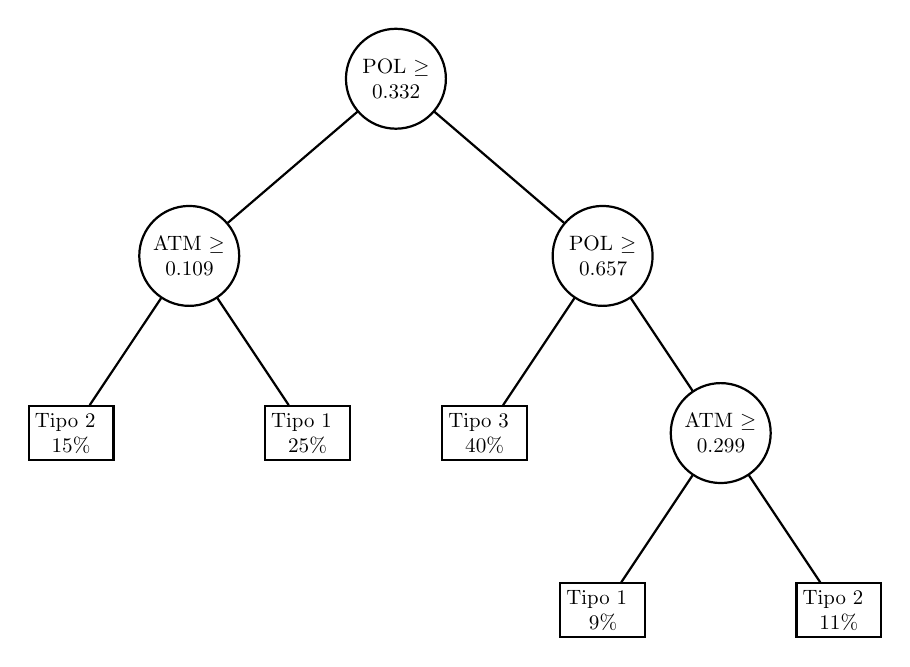
\begin{tikzpicture}[thick,scale=0.75, every node/.style={scale=0.75}]
\node [circle,draw,text width=1.2cm,align=center]{POL $\ge$ 0.332} [level distance=30mm,sibling distance=70mm]
child {node [circle,draw,text width=1.2cm,align=center] {ATM $\ge$ 0.109 } [level distance=30mm ,sibling distance=40mm]
child {node [rectangle,draw,text width=1.2cm,align=center] {Tipo 2\newline15\%}}
child {node [rectangle,draw,text width=1.2cm,align=center] {Tipo 1\newline25\%}}
}
child { node [circle,draw,text width=1.2cm,align=center]{ POL $\ge$ 0.657} [level distance=30mm ,sibling distance=40mm]
child {node [rectangle,draw,text width=1.2cm,align=center] {Tipo 3\newline40\%}}
child { node [circle,draw,text width=1.2cm,align=center]{ ATM $\ge$ 0.299 } [level distance=30mm ,sibling distance=40mm]
child {node [rectangle,draw,text width=1.2cm,align=center] {Tipo 1\newline9\%}}
child {node [rectangle,draw,text width=1.2cm,align=center] {Tipo 2\newline11\%}}
}
};
\end{tikzpicture}
\nota{Cada nó representa um atributo de um elemento da amostra. As folhas são consideradas a representação da classe a que uma observação pertence. Já o ramo é um conjunto de valores que reflete todas suas características e detalhes de um elemento}
\fonte{Criado pelo autor}
\end{figure}

\subsubsection{Árvore de regressão}

Para \citeonline[p. 307]{HASTIE}, árvores de regressão são utilizadas em problemas de predição. Assim, a variável de saída refere-se a uma variável numérica e contínua.

Assim como foi visto anteriormente, o algoritmo deve conseseguir decidir em quais variáveis e quais pontos as decisões serão tomadas, construindo a topologia da árvore.

No caso de uma regressão, poderia utiliza-se como critério de minimização a soma do mínimos quadrados \begin{math}\sum{ (y_{i} - f(x_{i}))^{2}}\end{math}, temos que o melhor \begin{math}\hat c_{m}\end{math} é exatamente a média para \begin{math}y_{i}\end{math} na região \begin{math}R_{m}\end{math}:

\begin{equation}
\label{eq:media}
\hat c_{m} = m\acute edia(y_{i} | x_{i} \in R_{m})
\end{equation}

Para encontrar a melhor partição, é necessário recorrer a um algoritmo guloso\footnotemark \footnotetext{\emph{algoritmo guloso} é um algoritmo que  busca a resolução de um problema elegendo sempre uma solução localmente ótima. Isto significa que, dentro de um conjunto de soluções possíveis numa determinada etapa da solução do problema, escolhe-se sempre a que traz o melhor resultado naquela situação, o que muitas vezes pode não levar a uma solução ótima global.}, uma vez que calcular utilizando os mínimos quadrados é computacionalmente inviável.

Seja \begin{math}j\end{math} uma variável de reparticionamento, $s$ um ponto de divisão. É possível definir um par de semi planos 

\begin{equation}
R_{1}(j,s) = {X | X_{j}\leq s} \quad \textrm{e} \quad R_{2}(j,s) = {X | X_{j}\textgreater s})
\end{equation}

Resultando a busca pela de \begin{math}s\end{math} e \begin{math}j\end{math} que resolva

\begin{equation}
\min_{j,s} \left [ \min_{c_{1}} \sum_{x_{i} \in R_{1} (j,s)} (y_{i} - c_{1})^{2} + \min_{c_{1}} \sum_{x_{i} \in R_{2} (j,s)}(y_{i} - c_{2})^{2} \right ]
\end{equation} 


Mas como visto em \ref{eq:media}, temos que para qualquer $j$ e $s$, a minimização interna pode ser resolvida por:

\begin{equation}
\hat c_{1} = m\acute edia(y_{i} | x_{i} \in R_{1}(j,s)) \quad \textrm{e} \quad \hat c_{2} = m\acute edia(y_{i} | x_{i} \in R_{2}(j,s))
\end{equation} 

Este processo é repetido até que todas as regiões sejam descobertas.

\subsubsection{Árvore de classificação}

Para o caso de uma árvore de classificação, \citeonline[p. 308]{HASTIE} explica que o objetivo principal concentra-se em conseguir, a partir das variáveis independentes, efetuar a decisão em definir um classe para uma determinada entrada de dados. Logo, a saída é uma variável categórica.
Neste caso, utiliza-se como critério de decisão o índice de Gini\footnotemark \footnotetext{Índice de Gini mede a frequencia de que um elemento selecionado aleatoriamente de um conjunto é marcado de forma errada}
\begin{math}Gini(T) = 1 - \sum_{i=1}^{n}{ p_{i}^{2}}\end{math},
onde p é a proporção de observações de uma determinada classe para um dado nó.

\subsection{\emph{Bagging}}

As árvores vistas anteriormente são modelos interessantes de classificação mas possuem um problema: o resultado gerado por elas em geral possuem uma acurácia muito baixa quando a estrutura da árvore começa a crescer muito \cite[p. 312]{HASTIE}.
A proposta do \emph{Bagging} é criar subconjuntos dos dados, gerando diversas árvores que deverão executar a classificação. Esses modelos subconjuntos são gerados com reposição, ou seja, um mesmo dado pode estar presente em mais de um modelo no momento do treino. Cada árvore gerada fornecerá um modelo para a \emph{Random Forest} e um valor intermediário será adotado para os nós. 

\begin{figure*}[ht!]
    \centering
        \caption{Exemplo de composição da \emph{Random Forest}}
    \begin{subfigure}[t]{0.5\textwidth}
        \centering
        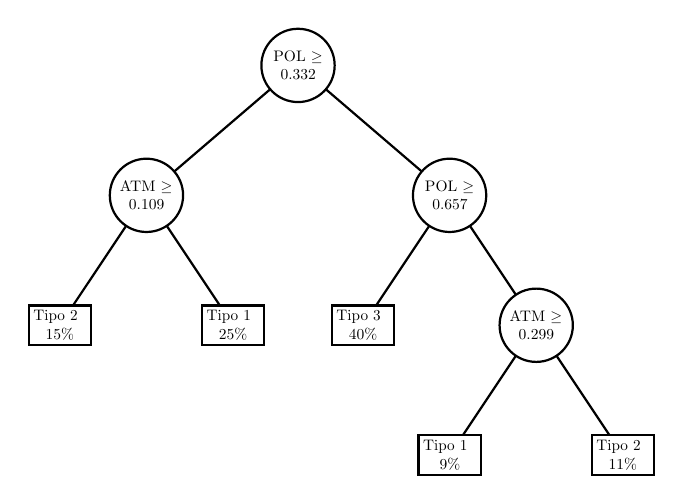
\begin{tikzpicture}[thick,scale=0.55, every node/.style={scale=0.55}]
\node [circle,draw,text width=1.2cm,align=center]{POL $\ge$ 0.332} [level distance=30mm,sibling distance=70mm]
child {node [circle,draw,text width=1.2cm,align=center] {ATM $\ge$ 0.109 } [level distance=30mm ,sibling distance=40mm]
child {node [rectangle,draw,text width=1.2cm,align=center] {Tipo 2\newline15\%}}
child {node [rectangle,draw,text width=1.2cm,align=center] {Tipo 1\newline25\%}}
}
child { node [circle,draw,text width=1.2cm,align=center]{ POL $\ge$ 0.657} [level distance=30mm ,sibling distance=40mm]
child {node [rectangle,draw,text width=1.2cm,align=center] {Tipo 3\newline40\%}}
child { node [circle,draw,text width=1.2cm,align=center]{ ATM $\ge$ 0.299 } [level distance=30mm ,sibling distance=40mm]
child {node [rectangle,draw,text width=1.2cm,align=center] {Tipo 1\newline9\%}}
child {node [rectangle,draw,text width=1.2cm,align=center] {Tipo 2\newline11\%}}
}
};
\end{tikzpicture}

        \caption{Configuração 1 da árvore de decisão}
    \end{subfigure}%
    ~ 
    \begin{subfigure}[t]{0.5\textwidth}
        \centering
        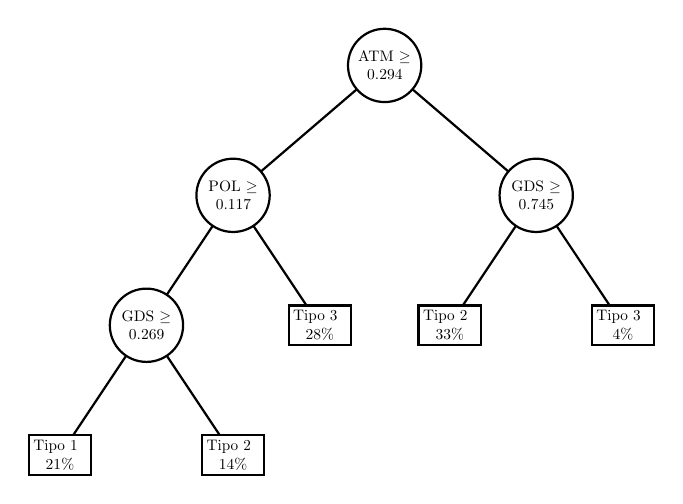
\begin{tikzpicture}[thick,scale=0.55, every node/.style={scale=0.55}]
\node [circle,draw,text width=1.2cm,align=center]{ATM $\ge$ 0.294} [level distance=30mm,sibling distance=70mm]
child { node [circle,draw,text width=1.2cm,align=center]{ POL $\ge$ 0.117 } [level distance=30mm ,sibling distance=40mm]
child { node [circle,draw,text width=1.2cm,align=center]{ GDS $\ge$ 0.269 } [level distance=30mm ,sibling distance=40mm]
child {node [rectangle,draw,text width=1.2cm,align=center] {Tipo 1\newline21\%}}
child {node [rectangle,draw,text width=1.2cm,align=center] {Tipo 2\newline14\%}}}
child {node [rectangle,draw,text width=1.2cm,align=center] {Tipo 3\newline28\%}}
}
child {node [circle,draw,text width=1.2cm,align=center] { GDS $\ge$ 0.745 } [level distance=30mm ,sibling distance=40mm]
child {node [rectangle,draw,text width=1.2cm,align=center] {Tipo 2\newline33\%}}
child {node [rectangle,draw,text width=1.2cm,align=center] {Tipo 3\newline4\%}}
};
\end{tikzpicture}
        \caption{Configuração 2 da árvore de decisão}
    \end{subfigure}
\fonte{Criado pelo autor}
\end{figure*}



% \begin{figure*}[t!]
%     \centering
%     \begin{subfigure}[t]{0.5\textwidth}
%         \centering
%         \begin{tikzpicture}[thick,scale=0.55, every node/.style={scale=0.55}]
% \node [circle,draw,text width=1.2cm,align=center]{POL $\ge$ 0.332} [level distance=30mm,sibling distance=70mm]
% child {node [circle,draw,text width=1.2cm,align=center] {ATM $\ge$ 0.109 } [level distance=30mm ,sibling distance=40mm]
% child {node [rectangle,draw,text width=1.2cm,align=center] {Tipo 2\newline15\%}}
% child {node [rectangle,draw,text width=1.2cm,align=center] {Tipo 1\newline25\%}}
% }
% child { node [circle,draw,text width=1.2cm,align=center]{ POL $\ge$ 0.657} [level distance=30mm ,sibling distance=40mm]
% child {node [rectangle,draw,text width=1.2cm,align=center] {Tipo 3\newline40\%}}
% child { node [circle,draw,text width=1.2cm,align=center]{ ATM $\ge$ 0.299 } [level distance=30mm ,sibling distance=40mm]
% child {node [rectangle,draw,text width=1.2cm,align=center] {Tipo 1\newline9\%}}
% child {node [rectangle,draw,text width=1.2cm,align=center] {Tipo 2\newline11\%}}
% }
% };
% \end{tikzpicture}

%         \caption{Configuração 1 da árvore de decisão}
%     \end{subfigure}%
%     ~ 
%     \begin{subfigure}[t]{0.5\textwidth}
%         \centering
%         \begin{tikzpicture}[thick,scale=0.55, every node/.style={scale=0.55}]
% \node [circle,draw,text width=1.2cm,align=center]{ATM $\ge$ 0.294} [level distance=30mm,sibling distance=70mm]
% child { node [circle,draw,text width=1.2cm,align=center]{ POL $\ge$ 0.117 } [level distance=30mm ,sibling distance=40mm]
% child { node [circle,draw,text width=1.2cm,align=center]{ GDS $\ge$ 0.269 } [level distance=30mm ,sibling distance=40mm]
% child {node [rectangle,draw,text width=1.2cm,align=center] {Tipo 1\newline21\%}}
% child {node [rectangle,draw,text width=1.2cm,align=center] {Tipo 2\newline14\%}}}
% child {node [rectangle,draw,text width=1.2cm,align=center] {Tipo 3\newline28\%}}
% }
% child {node [circle,draw,text width=1.2cm,align=center] { GDS $\ge$ 0.745 } [level distance=30mm ,sibling distance=40mm]
% child {node [rectangle,draw,text width=1.2cm,align=center] {Tipo 2\newline33\%}}
% child {node [rectangle,draw,text width=1.2cm,align=center] {Tipo 3\newline4\%}}
% };
% \end{tikzpicture}
%         \caption{Configuração 2 da árvore de decisão}
%     \end{subfigure}
%     \\
%     \centering
%     \begin{subfigure}[t]{0.5\textwidth}
%         \centering
%         \begin{tikzpicture}[thick,scale=0.55, every node/.style={scale=0.55}]
% \node [circle,draw,text width=1.2cm,align=center]{POL $\ge$ 0.332} [level distance=30mm,sibling distance=70mm]
% child {node [circle,draw,text width=1.2cm,align=center] {ATM $\ge$ 0.109 } [level distance=30mm ,sibling distance=40mm]
% child {node [rectangle,draw,text width=1.2cm,align=center] {Tipo 2\newline15\%}}
% child {node [rectangle,draw,text width=1.2cm,align=center] {Tipo 1\newline25\%}}
% }
% child { node [circle,draw,text width=1.2cm,align=center]{ POL $\ge$ 0.657} [level distance=30mm ,sibling distance=40mm]
% child {node [rectangle,draw,text width=1.2cm,align=center] {Tipo 3\newline40\%}}
% child { node [circle,draw,text width=1.2cm,align=center]{ ATM $\ge$ 0.299 } [level distance=30mm ,sibling distance=40mm]
% child {node [rectangle,draw,text width=1.2cm,align=center] {Tipo 1\newline9\%}}
% child {node [rectangle,draw,text width=1.2cm,align=center] {Tipo 2\newline11\%}}
% }
% };
% \end{tikzpicture}

%         \caption{Configuração 1 da árvore de decisão}
%     \end{subfigure}%
%     ~ 
%     \begin{subfigure}[t]{0.5\textwidth}
%         \centering
%         \begin{tikzpicture}[thick,scale=0.55, every node/.style={scale=0.55}]
% \node [circle,draw,text width=1.2cm,align=center]{ATM $\ge$ 0.294} [level distance=30mm,sibling distance=70mm]
% child { node [circle,draw,text width=1.2cm,align=center]{ POL $\ge$ 0.117 } [level distance=30mm ,sibling distance=40mm]
% child { node [circle,draw,text width=1.2cm,align=center]{ GDS $\ge$ 0.269 } [level distance=30mm ,sibling distance=40mm]
% child {node [rectangle,draw,text width=1.2cm,align=center] {Tipo 1\newline21\%}}
% child {node [rectangle,draw,text width=1.2cm,align=center] {Tipo 2\newline14\%}}}
% child {node [rectangle,draw,text width=1.2cm,align=center] {Tipo 3\newline28\%}}
% }
% child {node [circle,draw,text width=1.2cm,align=center] { GDS $\ge$ 0.745 } [level distance=30mm ,sibling distance=40mm]
% child {node [rectangle,draw,text width=1.2cm,align=center] {Tipo 2\newline33\%}}
% child {node [rectangle,draw,text width=1.2cm,align=center] {Tipo 3\newline4\%}}
% };
% \end{tikzpicture}
%         \caption{Configuração 2 da árvore de decisão}
%     \end{subfigure}
%     \caption{Configurações da árvore de decisão sobre subconjuntos distintos}
% \end{figure*}

Dessa forma, a solução para contornar esse problema foi a utilização dessa técnica nas árvores de decisões. Na \emph{Random Forest}, constrói-se uma árvore de classificação repetidamente usando amostras aleatórias do conjunto de dados. Por fim, o modelo final é recalculado.


% ---
% Conclusão
% ---
\chapter{Conclusão}
% ---
A regressão logística possui um comportamento mais estável, podendo ser facilmente usado em problemas que propicie uma separação linear dos dados. Eventualmente pode-se feature não lineares para que elas tenham um comportamento linear. Além disso, um dos problemas que pode ocorrer na regressão logística é o overfitting (existe tradução?) mas que pode ser contornado adicionando parâmetros l2 ou l1. Em situações em que é preciso lidar com um volume grande de dados (como ocorre com Big Data), a regressão logística permite o uso escalável utilizando recursos como ADMM. 

O Random forest possui vantagens como a possibilidade de trabalhar com base de dados que não tenham um comportamento linear. Além disso, elas podem tratar variáveis categóricas, fato que é complicado quando se trabalha com regressão logística (até possui um tratamento para tal (transformar a variável categórica em variáveis dummies) mas que pode tornar o cálculo mais complexo), já que o random forest são árvores de decisões. Com o uso de bagging ou boosting, é possível trabalhar com uma grande quantidade de variáveis, além de realizar diversos treinos. Além disso, a random forest pode selecionar quais são as variáveis mais relevantes independente da quantidade de váriaveis que ela receba inicialmente.




%\lipsum[31-33]


% ---
% Conclusão
% ---
\chapter{Conclusão}
% ---
A regressão logística possui um comportamento mais estável, podendo ser facilmente usado em problemas que propicie uma separação linear dos dados. Eventualmente pode-se feature não lineares para que elas tenham um comportamento linear. Além disso, um dos problemas que pode ocorrer na regressão logística é o overfitting (existe tradução?) mas que pode ser contornado adicionando parâmetros l2 ou l1. Em situações em que é preciso lidar com um volume grande de dados (como ocorre com Big Data), a regressão logística permite o uso escalável utilizando recursos como ADMM. 

O Random forest possui vantagens como a possibilidade de trabalhar com base de dados que não tenham um comportamento linear. Além disso, elas podem tratar variáveis categóricas, fato que é complicado quando se trabalha com regressão logística (até possui um tratamento para tal (transformar a variável categórica em variáveis dummies) mas que pode tornar o cálculo mais complexo), já que o random forest são árvores de decisões. Com o uso de bagging ou boosting, é possível trabalhar com uma grande quantidade de variáveis, além de realizar diversos treinos. Além disso, a random forest pode selecionar quais são as variáveis mais relevantes independente da quantidade de váriaveis que ela receba inicialmente.




%\lipsum[31-33]



% ----------------------------------------------------------
% ELEMENTOS PÓS-TEXTUAIS
% ----------------------------------------------------------
\postextual
% ----------------------------------------------------------

% ----------------------------------------------------------
% Referências bibliográficas
% ----------------------------------------------------------
\bibliography{abntex2-modelo-references}

% ----------------------------------------------------------
% Glossário
% ----------------------------------------------------------
%
% Consulte o manual da classe abntex2 para orientações sobre o glossário.
%
%\glossary

% ---
% Conclusão
% ---
\chapter{Conclusão}
% ---
A regressão logística possui um comportamento mais estável, podendo ser facilmente usado em problemas que propicie uma separação linear dos dados. Eventualmente pode-se feature não lineares para que elas tenham um comportamento linear. Além disso, um dos problemas que pode ocorrer na regressão logística é o overfitting (existe tradução?) mas que pode ser contornado adicionando parâmetros l2 ou l1. Em situações em que é preciso lidar com um volume grande de dados (como ocorre com Big Data), a regressão logística permite o uso escalável utilizando recursos como ADMM. 

O Random forest possui vantagens como a possibilidade de trabalhar com base de dados que não tenham um comportamento linear. Além disso, elas podem tratar variáveis categóricas, fato que é complicado quando se trabalha com regressão logística (até possui um tratamento para tal (transformar a variável categórica em variáveis dummies) mas que pode tornar o cálculo mais complexo), já que o random forest são árvores de decisões. Com o uso de bagging ou boosting, é possível trabalhar com uma grande quantidade de variáveis, além de realizar diversos treinos. Além disso, a random forest pode selecionar quais são as variáveis mais relevantes independente da quantidade de váriaveis que ela receba inicialmente.




%\lipsum[31-33]


% ---
% Conclusão
% ---
\chapter{Conclusão}
% ---
A regressão logística possui um comportamento mais estável, podendo ser facilmente usado em problemas que propicie uma separação linear dos dados. Eventualmente pode-se feature não lineares para que elas tenham um comportamento linear. Além disso, um dos problemas que pode ocorrer na regressão logística é o overfitting (existe tradução?) mas que pode ser contornado adicionando parâmetros l2 ou l1. Em situações em que é preciso lidar com um volume grande de dados (como ocorre com Big Data), a regressão logística permite o uso escalável utilizando recursos como ADMM. 

O Random forest possui vantagens como a possibilidade de trabalhar com base de dados que não tenham um comportamento linear. Além disso, elas podem tratar variáveis categóricas, fato que é complicado quando se trabalha com regressão logística (até possui um tratamento para tal (transformar a variável categórica em variáveis dummies) mas que pode tornar o cálculo mais complexo), já que o random forest são árvores de decisões. Com o uso de bagging ou boosting, é possível trabalhar com uma grande quantidade de variáveis, além de realizar diversos treinos. Além disso, a random forest pode selecionar quais são as variáveis mais relevantes independente da quantidade de váriaveis que ela receba inicialmente.




%\lipsum[31-33]




%---------------------------------------------------------------------
% INDICE REMISSIVO
%---------------------------------------------------------------------
\phantompart
\printindex
%---------------------------------------------------------------------

\end{document}
